\section{Máquinas de vectores soporte}

\paragraph{Introducción}

Para más información sobre la clasificación, consultar el último capítulo de \citep{ApuntesEstII}.
%

Disponemos de una muestra de datos bien clasificados (\textit{training data}):

\[
(x_1,y_1),\ldots, (x_n,y_n)
\]
donde $x_i\in \mathbb{R}^d$ son las variables observadas e $y_i\in\{-1,1\}$ es la etiqueta que representa la clase a la que pertenecen las observaciones.

\

Se observa ahora un nuevo vector $x$ independiente de los anteriores.

El objetivo es determinar a qué clase pertenece la observación $x$.

\

La regla óptima (regla Bayes) consiste en asignar a $x$ el valor $y=1$ si y solo si
\[
\mathbb{P}(y=1| x) > \mathbb{P}(y=-1|x)
\]
No es aplicable en la práctica, con lo que necesitamos buscar otros sistemas. 
%
A lo largo de este tema vamos a estudiar una regla de clasificación basada en contenidos anteriores del curso.

\paragraph{SVM para datos separables}

Suponemos que las muestras de ambos grupos son separables mediante un hiperplano:

\begin{figure}[hbtp]
\centering
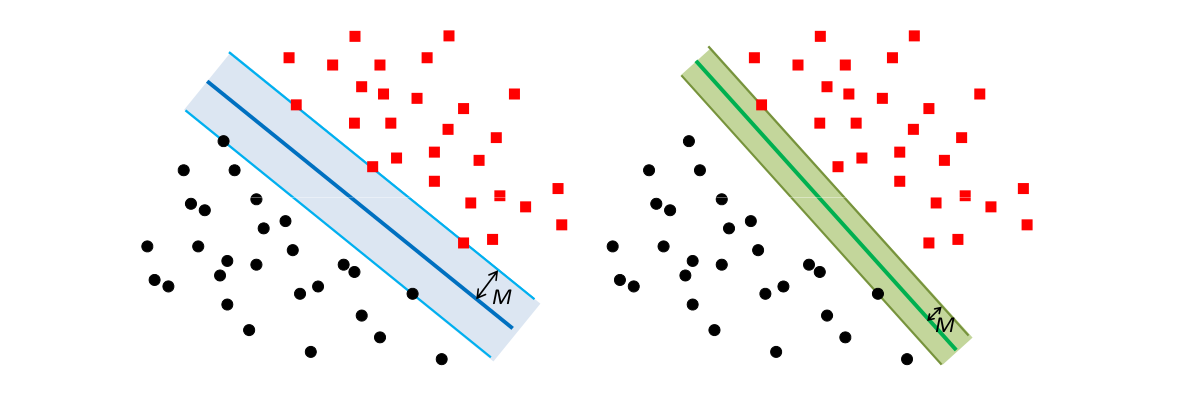
\includegraphics[scale=0.7]{img/margen}
\caption{Datos separables}
\end{figure}

El \concept{margen} de un hiperplano separador viene dado por la menor distancia de los puntos al hiperplano. 

El \concept{hiperplano óptimo} es aquel que maximiza el margen.


Dada una muestra de datos $(x_i,y_i)$, para poder clasificarla necesitamos encontrar ese hiperplano separador.
%
Definimos las clases $y_i\in\{-1,1\}$. Entonces, un hiperplano separador verifica $y_i(ω'x_i+ω_0)>0$.
%
Si es de clase $y_i=-1$, entonces $(ω'x_i + ω_0) < 0$ y viceversa.

Pdemos definir $ω$ y $ω_0$ de manera que  $\min_i \{y_i(w' x_i + w_0)\}=1$
con lo que el margen es: $\mbox{Margen} = \min_i  \frac{y_i(w' x + w_0)}{\|w\|} = \frac{1}{\|w\|}$.


\paragraph{Cálculo de hiperplano óptimo}


Para buscar el hiperplano óptimo, que es aquel que maximiza el márgen. Entonces, el problema de optimización asociado es:

\begin{ioprob}
\goal{$\min \frac{\norm{ω}^2}{2}$}
\restrictions{$y_i(ω'x_i + ω_0) ≥ 1$}{}{}{}{}{}
\end{ioprob}


Al resolver este problema, por la holgura complementaria, llegamos  a que el óptimo sólo depende de los puntos en los que $u_i≠0 \to y_i(ω'x_i + ω_0) = 1$, es decir, en la frontera.

\subparagraph{Cálculo del dual}
Vamos a estudiar el problema dual del planteado aquí.

\[
	g(u) = \frac{1}{2} \underbrace{\left(\sum_i y_iu_ix_i\right)^\top}_{ω} \underbrace{\sum_jy_ju_jx_j}_{ω} - \sum u_jy_jx_j\right)^\top x_i - \left(\sum y_ju_j\right)ω_0 + \sum u_i = \sum_{i=1}^n u_i - \frac{1}{2} \sum_{i=1}^n \sum_{j=1}^n  u_i u_j y_i y_j x'_i x_j 
\]

Con lo que:

\[
	g(u) =\begin{array}{ccc} -∞ & si &\sum y_iu_i ≠ 0\\ \sum u_i - \frac{1}{?}\sum_i\sum_j u_i u_j y_i y_j x'_i x_j  & si & \sum y_iu_i = 0
	\end{array}
\]

Vamos a expresar el problema dual.
%
Tomando $\vec{1} = (1,...,1)$, y $H = (h_{ij}) = (y_iy_jx'_ix_j)$

\begin{ioprob}
\goal{$\max \vec{1}^\top u - \frac{1}{2}\vec{u}^\top H\vu$}
\restrictions{$\vy^\top \vu = 0$}{$u≥0$}{}{}{}{}
\end{ioprob}

¿Es este problema convexo? Para poder contestar necesitaríamos que $H$ sea semidefinida positiva. 
%
Esto es cierto porque:

\[
	\vu'H\vu = \norm{\sum ...}^2 ≥ 0
\]


Como $H$ es semidefinida positiva, tenemos un problema convexo. \todo{¿Porqué?}

Además, \textbf{la solución depende} de $x_1,\ldots,x_n$ \textbf{únicamente a través de los productos escalares} $x'_ix_j$.


\subparagraph{Holgura complementaria}

A partir de la solución del dual, $\hat u$, aplicamos $\hat w = \sum_{i=1}^n \hat u_i y_i x_i$ para obtener $\hat w$.

 Sean $S=\{i:\, \hat u_i>0\}$ los índices de los vectores soporte.
Por las condiciones de holgura complementaria,  para cada $i\in S$,
\[
\hat w_0 = \frac{1-y_i\hat w'x_i}{y_i} = y_i-\hat w'x_i.
\] 


En la práctica, es numéricamente más estable usar el promedio de estos valores. Si $\# S=n_s$.
\[
\hat w_0 = \frac{1}{n_s} \sum_{i\in S} (y_i-\hat w'x_i).
\]

\subsubsection{Regla de clasificación}

Resulta una regla de clasificación lineal: asignamos a $x$ el valor $y=1$ si y solo si $\hat{w}'x+\hat w_0>0$.

\

\[
\hat w_0 + \hat{w}'x>0 \Leftrightarrow \hat w_0 + \left[\sum_{i\in S} y_i \hat u_i x_i\right]' x > 0 
\]

\

Si $\alpha_i=y_i\hat u_i$, también podemos escribir la regla de clasificación como:
\[
y = 1 \Leftrightarrow  \hat w_0 + \sum_{i\in S} \alpha_i (x'_ix)>0
\]

¿Cómo afecta a la clasificación una rotación de los datos?

Tomamos $\tilde{u}_i = Cu_i$, siendo $C$ ortonormal. 
%
Repasando los cálculos anteriores con $\tilde{u}_i$ obtenemos que $\tilde{ω} = Cω$, es decir, el hiperplano óptimo de los datos rotados es la rotación del hiperplano óptimo.

\paragraph{SVM datos no separables}

En la realidad, los datos separables no son habituales. 
%
El truco es añadir una penalización a los puntos que están mal clasificados (o demasiado cerca del hiperplano). Es decir:

\[
	y_i(ω'x_i + ω_0) ≥ 1-\xi_i
\]

¿Cuánto penalizamos la distancia? Eso se refleja con una constante $C$, de la siguiente manera:

\begin{ioprob}
\goal{$\|w\|^2 / 2 + C\sum_{i=1}^n \xi_i$}
\restrictions{$y_i(w' x_i + w_0) + \xi_i\geq 1\;\; i=1,\ldots,n$}{$\xi_i\geq 0\;\;i=1,\ldots,n$}{}{}{}{}
\end{ioprob}

Y ahora, para construir la regla de clasificación damos los mismos pasos que en el caso de datos separables linealmente. 
%
Estos son: $KKT$, problema dual, holgura complementaria.

\todoby{dejuan}

Llegamos al problema dual:


\begin{ioprob}
\goal{$\max g(u) = \vec{1}'\vu - \rfrac{1}{2}\vec{u}'H\vu$}
\restrictions{$\vu'y = 0$}{$C≥u≥0$}{}{}{}{}
\end{ioprob}

La única diferencia que aparece es $C≥u$, es decir, los pesos están acotados superiormente.
